% SIAM Article Template
\documentclass[review,onefignum,onetabnum]{siamonline190516}

% Information that is shared between the article and the supplement
% (title and author information, macros, packages, etc.) goes into
% ex_shared.tex. If there is no supplement, this file can be included
% directly.

% SIAM Shared Information Template
% This is information that is shared between the main document and any
% supplement. If no supplement is required, then this information can
% be included directly in the main document.


% Packages and macros go here
\usepackage{lipsum}
\usepackage{amsfonts}
\usepackage{graphicx}
\usepackage{epstopdf}
\usepackage{algorithmic}
%\usepackage{algpseudocode}
%\usepackage{array} % <- Preamble 
%\usepackage{subfig} % <- Preamble

%\usepackage{amsmath}
%\usepackage{mathtools}
\usepackage{cleveref}
\usepackage{bm}
\usepackage{mathrsfs}
\usepackage{placeins}
%\usepackage{tcolorbox}
%\usepackage{caption}
%\usepackage{subcaption}
%\usepackage[]{algorithm2e}
%\usepackage{amsthm}
\usepackage{url} % to cite webpage
\usepackage[utf8]{inputenc}
%\newtcolorbox{satbox}{colback=green!5!white,colframe=green!75!black}
%\newtcolorbox{jacbox}{colback=yellow!5!white,colframe=yellow!75!black}
%\newtheorem{definition}{Definition}
%\newtheorem{remark}{Remark}
%\newtheorem{proposition}{Proposition}
%\newtheorem{lemma}{Lemma}


\ifpdf
  \DeclareGraphicsExtensions{.eps,.pdf,.png,.jpg}
\else
  \DeclareGraphicsExtensions{.eps}
\fi

% Prevent itemized lists from running into the left margin inside theorems and proofs
\usepackage{enumitem}
\setlist[enumerate]{leftmargin=.5in}
\setlist[itemize]{leftmargin=.5in}

% Add a serial/Oxford comma by default.
\newcommand{\creflastconjunction}{, and~}

% Used for creating new theorem and remark environments
\newsiamremark{remark}{Remark}
\newsiamremark{hypothesis}{Hypothesis}
\crefname{hypothesis}{Hypothesis}{Hypotheses}
\newsiamthm{claim}{Claim}
%Continuous
\newcommand{\vecs}[1]{\vec{\mskip\thinmuskip #1}}
\newcommand{\wc}{\vecs{w}}
\newcommand{\xic}{\vecs{\xi}}
\newcommand{\wcn}{w_n}
\newcommand{\wct}{w_s}
\newcommand{\uc}{u}
\newcommand{\vc}{v}
\newcommand{\phic}{\vecs{\phi}}
\newcommand{\psic}{\vecs{\psi}}
\newcommand{\nc}{\vecs{n}}
\renewcommand{\div}{{\nabla\cdot}}
\newcommand{\dOmega}{{\partial\Omega}}
\newcommand{\ipc}[2]{\left(#1, #2\right)_\Omega} %Inner product on Omega
\newcommand{\ipbc}[2]{\left(#1, #2\right)_{\partial \Omega}} %Inner product on dOmega
\newcommand{\ipbcpart}[2]{\left(#1, #2\right)_{\Gamma_d}} %Inner product on dOmega
\newcommand{\ipgd}[2]{\left(#1, #2\right)_{\Gamma_d}} %Inner product on Gamma_d
\newcommand{\normc}[1]{\|#1\|_\Omega}


%Discrete
\newcommand{\wn}{\vecs{\bm{w}}}
\newcommand{\wnn}{\bm{w}_n}
\newcommand{\wtn}{\bm{w}_s}
\newcommand{\un}{\bm{u}}
\newcommand{\vn}{\bm{v}}
\newcommand{\pn}{\bm{p}}
\newcommand{\fn}{\bm{f}}
\newcommand{\gn}{\bm{g}}
\newcommand{\en}{\bm{e}}
\newcommand{\xn}{\bm{x}}
\newcommand{\xin}{\vecs{\bm{\xi}}}
\newcommand{\phin}{\vecs{\bm{\phi}}}
\newcommand{\psin}{\vecs{\bm{\psi}}}
\newcommand{\zeron}{\bm{0}}
\newcommand{\In}{\bm{I}}
\newcommand{\nn}{\vecs{\bm{n}}}
\newcommand{\nnx}{\bm{n}_x}
\newcommand{\nny}{\bm{n}_y}
\newcommand{\nablan}{\bm{\nabla}}
\newcommand{\divn}{\bm{\nabla\cdot}}
\newcommand{\Dx}{\bm{D_x}}
\newcommand{\Dy}{\bm{D_y}}
\newcommand{\Pn}{\bm{P}}
\newcommand{\Png}{\bm{P}_d}
\newcommand{\Ln}{\bm{L}}
\newcommand{\Lng}{\bm{L}_d}
\newcommand{\Pncal}{\bm{\mathcal{P}}}
\newcommand{\ipn}[2]{\left(#1, #2\right)_{\Omega_h}} %Discrete inner product on Omega
\newcommand{\normn}[1]{\|#1\|_{\Omega_h}}
\newcommand{\ipbn}[2]{\left(#1, #2\right)_{\Gamma_d}} %Discrete inner product on Gamma
\newcommand{\ipbnfull}[2]{\left(#1, #2\right)_{\partial \Omega_h}} %Discrete inner product on Gamma
\newcommand{\euln}{\bm{\mathcal{L}}}
\newcommand{\satn}{\bm{\mathcal{S}}}
\newcommand{\Hn}{\bm{\mathcal{H}}}
\newcommand{\Fn}{\bm{\mathcal{F}}}
\newcommand{\Mn}{\mathcal{M}}
\newcommand{\diagn}[1]{\underline{#1}}
\newcommand{\soln}{\bm{\chi}}
\newcommand{\cdotn}{\bm{\cdot}}


% Sets running headers as well as PDF title and authors
\headers{An Explicit Jacobian}{F. Laur\'en, O. $\rm \mathring{A}$lund, and J. Nordstr\"om}

% Title. If the supplement option is on, then "Supplementary Material"
% is automatically inserted before the title.
\title{An Explicit Jacobian for Newton's Method Applied to Numerical Approximations of Nonlinear Initial Boundary Value Problems\thanks{Submitted to the editors \today.
\funding{This work was funded by the Swedish Research Council (Stokcholm) under grant number 2018-05084\_VR} and SESSI.}}

% Authors: full names plus addresses.
\author{Fredrik Laur\'en\thanks{Department of Mathematics, Computational Mathematics, Link\"oping University, SE-581 83 Link\"oping, Sweden 
(\email{fredrik.lauren@liu.se}),(\email{oskar.alund@liu.se}), (\email{jan.nordstrom@liu.se}).}
\and Oskar $\rm \mathring{A}$lund \footnotemark[2]
\and Jan Nordstr\"om \footnotemark[2]\ \thanks{Department of Mathematics and Applied Mathematics, University of Johannesburg,P.O. Box 524, Auckland Park 2006, South Africa}.}

\usepackage{amsopn}
\DeclareMathOperator{\diag}{diag}


%%% Local Variables: 
%%% mode:latex
%%% TeX-master: "ex_article"
%%% End: 


% Optional PDF information
%\ifpdf
%\hypersetup{
%  pdftitle={test.pdf},
%  pdfauthor={F. Laur\'en, O. $\rm \mathring{A}$lund, and J. Nordstr\"om}}
%\fi

% The next statement enables references to information in the
% supplement. See the xr-hyperref package for details.

\externaldocument{ex_supplement}

% FundRef data to be entered by SIAM
%<funding-group specific-use="FundRef">
%<award-group>
%<funding-source>
%<named-content content-type="funder-name"> 
%</named-content> 
%<named-content content-type="funder-identifier"> 
%</named-content>
%</funding-source>
%<award-id> </award-id>
%</award-group>
%</funding-group>

\begin{document}

\maketitle

% REQUIRED
\begin{abstract}
We derive an explicit form of the Jacobian for discrete approximations of nonlinear initial boundary value problems (IBVPs) on matrix-vector form. The technique is exemplified on the incompressible Navier-Stokes equations in two dimensions. The Jacobian facilitates the use of Newton's method to solve the corresponding nonlinear system of equations. Appropriate boundary conditions are weakly imposed  and we show how to compute the Jacobian for those parts of the discretization as well. The convergence rate of the iterations is verified by using the method of manufactured solutions. The methodology in this paper that can be used on any numerical discretization of IBVPs on matrix-vector form.
\end{abstract}

% REQUIRED
\begin{keywords}
 Nonlinear initial boundary value problems, Jacobian, Newton's method, incompressible Navier-Stokes equations, summation-by-parts, weak boundary conditions.
\end{keywords}

% REQUIRED
%see here: https://mathscinet.ams.org/mathscinet/msc/msc2020.html?t=65Mxx&btn=Current
\begin{AMS}
  65M06, 65M12
\end{AMS}

\section{Introduction}%
\label{sec:introduction}

Discretizing partial differential equations revolves around three major considerations:
\begin{enumerate}
  \item Stability
  \item Simplicity
  \item Efficiency
\end{enumerate}
These aspects continually compete for attention, and narrow focus on one of them is often detrimental to the other two. This paper is an attempt to strike a balance between the three in the context of the incompressible Euler equations. Point 1 (stability) is achieved by using well established techniques, such as weakly imposed boundary conditions and integration-by-parts mimicking discrete differential operators. Point 2 (simplicity) is achieved through a convenient notational structure that closely resembles the continuous notation both functionally and visually. Our ambition is to narrow the bridge between the continuous and discrete settings as much as possible so that understanding of the continuous problem transfers with little effort to the discrete problem. Point 3 (efficiency) is achieved using two key tools: encapsulation and explicit Jacobians. By encapsulation we mean that the discrete derivative operators can be thought of as abstract operators that act on discrete approximations of differentiable functions, while satisfying certain key properties (most notably accuracy and summation-by-parts). Such abstraction is useful, not only because it simplifies stability proofs, but also because it isolates concerns: Discrete differentiation can be implemented, optimized, and maintained in separation from any particular solver. Encapsulation also allows us to write down, in very compact form, explicit Jacobians for the discretized incompressible Euler equations in terms of the derivative operators. 

Explicit Jacobians are particularly powerful in the context of implicit timestepping since they are typically orders of magnitude faster to evaluate than for example a finite difference based approximation of the Jacobian. Altough we in this paper consider the incompressible Euler equations in two dimensions, the framework can be extended to any type of hyperbolic or parabolic equations.


\section{Problem formulation}\label{sec:continuous}
As an illustrative example of our technique, we consider the scenario illustrated in \cref{fig:domain}. 
\begin{figure}%
  \centering
  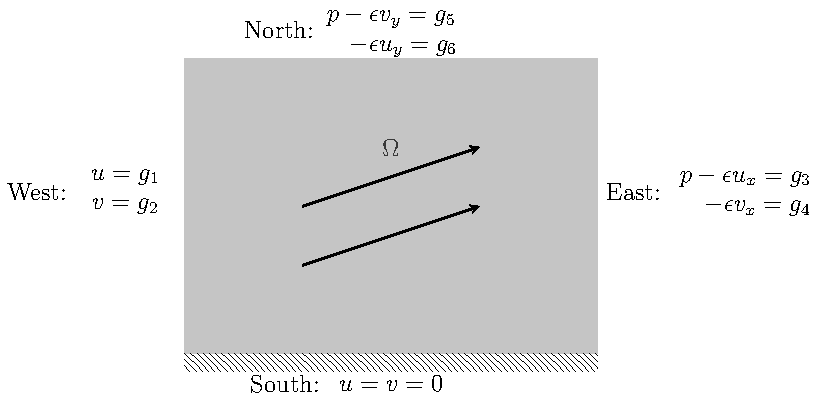
\includegraphics[width=0.7\textwidth]{images/domain/domain.pdf}
  \caption{Illustration of the computational domain $\Omega$ and the specific boundary conditions.}%
  \label{fig:domain}
\end{figure}
An incompressible fluid is moving from left to right. Hence, the left side is an inflow boundary, where Dirichlet conditions are imposed, and the right side is an outflow boundary, where natural boundary conditions \cite{papanastasiou1992new} are imposed. The lower part of the domain is a no-slip wall and the upper side is an outflow boundary, where again natural conditions are imposed. The initial-boundary value problem for the INS equations that we consider is
\begin{equation}
\begin{aligned}
  \tilde{I} \w_t  + \eul(\w)	& = 0
	& \quad & (x,y) \in \Omega, & \quad t & > 0
	\\
	\mathcal{H} \w & =  \g & \quad & (x,y) \in \partial\Omega, & \quad t & > 0
	\\
  \tilde{I} \w 	& =  \tilde{I}\f & \quad & (x,y) \in \Omega, & \quad t & = 0
	\, .
\end{aligned} 
\label{eq:ins_continuous}
\end{equation}
In \eqref{eq:ins_continuous}, $\w = (u,v,p)^\top$, where $u,v$ are the velocities in the $x,y$ direction, respectively, and $p$ is the pressure. Furthermore, $\Omega = [0,1]^2$ is the domain and $\partial \Omega$ its boundary. The initial data $\f$ and boundary data $\g$ are sufficiently smooth and compatible functions and the spatial operator is given by \cite{nordstrom2019energy}
\begin{equation}
  \eul(\w) = 
  \frac{1}{2}\left[A \w_x + (A \w)_x + B \w_y + (B \w)_y\right] 
  - \epsilon\tilde{I}[\w_{xx} + \w_{yy}]
  \, .
  \label{eq:eul}
\end{equation}
The matrices in \eqref{eq:ins_continuous} and $\eqref{eq:eul}$ are 
\[
   A = 
   \begin{pmatrix}
      u & 0 & 1
      \\
      0 & u & 0
      \\
      1 & 0 & 0
   \end{pmatrix}
   , \quad 
   B = 
   \begin{pmatrix}
      v & 0 & 0
      \\
      0 & v & 1
      \\
      0 & 1 & 0
   \end{pmatrix}
   ,\quad 
   \tilde{I} = 
   \begin{pmatrix}
      1 & 0 & 0
      \\
      0 & 1 & 0
      \\
      0 & 0 & 0
   \end{pmatrix}
   \, .
\]
Lastly, the explicit form of the boundary conditions $\mathcal{H}\w = \g$ reads
\begin{equation}
\begin{aligned}
  u & = g_1 \quad & v & = g_2  & \quad & \text{at}  \quad x = 0 \quad && \text{(West)}
  \\
  p - \epsilon u_x & = g_3 \quad & -\epsilon v_x & = g_4 & \quad & \text{at} \quad x = 1  \quad && \text{(East)}
  \\
  u &= 0 \quad & v &= 0        & \quad & \text{at}  \quad y = 0 \quad && \text{(South)}
  \\
  p-\epsilon v_y &= g_5 \quad & -\epsilon u_y &= g_6        & \quad & \text{at}  \quad y = 1 \quad && \text{(North)}
  \, .
\label{eq:boundary_conditions}
\end{aligned}
\end{equation}

\subsection{Boundedness}
We will for completeness show how to bound the solution. For simplicity, only the south side of the domain is discussed explicitly. Details of the upcoming analysis are found in \cite{nordstrom2019energy}. 

For two vector functions $\phiv,\psiv$ defined on $\Omega$, we introduce the inner product and norm
\[
  \langle \phiv, \psiv \rangle = \int_\Omega \phiv^\top \psiv d\Omega
  , \quad
  \|\phiv\|^2 = \langle \phiv,\phiv\rangle
  \, .
\]
By multiplying \eqref{eq:ins_continuous} by $2\w^\top$ from the left and integrating over $\Omega$, we get
\begin{equation}
   \frac{d}{dt}\|\w\|^2_{\It} + 2\epsilon \|\nabla \w\|^2_{\It} =  BT
   \, ,
   \label{eq:energy_continuous}
\end{equation}
where $\nabla \w = (\nabla u,\nabla v, \nabla p)^\top$, $\|\nabla \w\|^2_{\It}$ is a dissipative volume term and
\[
  BT = 
  \int_{\text{South}}\w^\top (B \w - 2\epsilon \It \w_y) d x
\]
contains the boundary terms evaluated at the south boundary. The other boundary terms are assumed dissipative and ignored. Imposing $u = v = 0$ results in $BT = 0$. Integrating \eqref{eq:energy_continuous} in time (assuming homogeneous boundary conditions on all sides) leads to 
\begin{equation}
   \|\w\|^2_{\tilde{I}}(T) + 2\epsilon \int_0^T\|\nabla \w\|^2_{\tilde{I}} dt
   \le  \|f\|_{\tilde{I}}^2
   \, ,
   \label{eq:estimate_continuous}
\end{equation}
which bounds the semi-norm of the solution ($\|\w\|^2_{\tilde{I}}$) and its gradients ($\|\nabla \w\|^2_{\tilde{I}}$) for any time.

\section{The semi-discrete scheme}\label{sec:semi_discrete}
A brief introduction of the SBP-SAT technique is provided below and we recommend \cite{fernandez2014review,svard2014review} for extensive reviews. 

We discretize the domain $\Omega = [0,1]^2$ with $N+1$ and $M+1$ grid points; $x_i = i/N$, $i = 0,\dots, N$ and $y_j = j/M$, $j= 0,\dots,M$ and let $n = (N+1)(M+1)$ denote the total number of grid points. A scalar function $q = q(x,y)$ defined on $\Omega$ is thereby represented on the grid by $\qn = (q_{00}, \dots, q_{0M}, \dots q_{N0},\dots q_{NM})^\top$ where $q_{ij} = q(x_i,y_j)$. For the vector-valued function $\vecs{w} = (u,v,p)^\top$, the approximation is arranged as $\wn = (\un^\top,\vn^\top,\pn^\top)^\top$.
Let $\Dx = (P^{-1}_x Q_x) \otimes I_{M+1}$ and $\Dy = I_{N+1} \otimes (P^{-1}_y Q_y)$, where $\otimes$ denotes the Kronecker product. Then the approximations of the spatial derivatives are given by 
\[
  \Dx \un \approx \un_x,
  \quad 
  \Dy \un \approx \un_y
  \, .
\]
The matrices $P_{x,y}$ are diagonal and positive definite, so that $\Pn = P_x\otimes P_y$ forms a quadrature rule that defines the norm $\|\wn\|^2_{I_3\otimes\Pn} = \wn^\top (I_3\otimes\Pn) \wn \approx \iint_\Omega \vecs{w}^\top \vecs{w} d\Omega$. We have also introduced $I_{k}$, which is the identity matrix of size $k$. Moreover, the matrices $Q_{x,y}$ satisfy the SBP-property 
\begin{equation}
  Q_{x} + Q_{x}^\top = E_N - E_{0x}
  \quad 
  Q_{y} + Q_{y}^\top = E_M - E_{0y}
  \, ,
  \label{eq:sbp_property}
\end{equation}
where $E_{0x,y} = \text{diag}(1,0,0, \dots,0)$ and $E_{N,M} = \text{diag}(0,0,0,\dots,1)$ are matrices of appropriate sizes.

By using the notation above, the semi-discrete approximation of \eqref{eq:ins_continuous} becomes \cite{nordstrom2019energy}
\begin{equation}
  \label{eq:ins_semi_discrete}
  \Itn \wn_t  + \euln(\wn) = \satn(\wn) \, .
\end{equation}
The discrete spatial operator is given by
\begin{equation*}
\begin{aligned}
  \euln(\wn) &=
  \frac{1}{2}\left[\An (I_3\otimes \Dx)\wn + (I_3\otimes \Dx) \An\wn +
                   \Bn (I_3\otimes \Dy)\wn + (I_3\otimes \Dy) \Bn\wn\right]
  \\
  & - \epsilon \Itn [(I_3\otimes \Dx)^2 + (I_3\otimes \Dy)^2]\wn \, ,
\end{aligned}
\end{equation*}
and the block matrices are
\[
  \An = 
  \begin{pmatrix}
    \Un & \zeron & \In 
    \\
    \zeron  & \Un & \zeron
    \\
    \In & \zeron & \zeron
  \end{pmatrix}
  ,
  \quad 
  \Bn = 
  \begin{pmatrix}
    \Vn &  \zeron & \zeron 
    \\
    \zeron  & \Vn & \In
    \\
    \zeron & \In & \zeron
  \end{pmatrix}
  ,
  \quad
  \Itn = 
  \begin{pmatrix}
    \In &  \zeron & \zeron 
    \\
    \zeron  & \In & \zeron
    \\
    \zeron & \zeron & \zeron
  \end{pmatrix}
  \, ,
\]
where $\Un,\Vn \in \Rbb^{n\times n}$ are diagonal matrices holding $\un,\vn$, respectively. The matrices $\In$ and $\zeron$ are the identity and the zero matrix of size $n\times n$. Furthermore, $\satn(\wn)$ contains penalty terms that enforce the boundary conditions. 

The purpose of the SAT $\satn(\wn)$ is $i)$ to enforce the boundary conditions in \eqref{eq:boundary_conditions} and $ii)$ to stabilize the solution. 
One penalty term for each of the boundary conditions in \eqref{eq:boundary_conditions} will be constructed. Let $k\in\{W,E,S,N\}$. The SAT at boundary $k$ that enforces the boundary condition $H^k\vecs{w} = \g$ has the general form
\begin{equation}
  \satn^k(\wn) = (I_3\otimes\Pn^{-1})\Sigma^k(I_3\otimes\Pn^{k})(\Hn^k\wn - \vec{\gn})
  \, .
  \label{eq:penalty_general}
\end{equation}
In \eqref{eq:penalty_general}, $\Sigma^k$ is the penalty matrix to be determined for stability at boundary $k$. The quadratures are
\begin{equation*}
	\Pn^k = 
	\begin{cases}
    E_{0x}\otimes P_y 	\quad 	& \text{on the west boundary } (k = W)
		\\
    E_N\otimes P_y 	\quad  	& \text{on the east boundary } (k = E)
		\\
    P_x\otimes E_{0y} 	\quad  	& \text{on the south boundary } (k = S)
		\\
		P_x\otimes E_M 	\quad  	& \text{on the north boundary } (k = N)
    \, .
	\end{cases}
\end{equation*}

For the boundary conditions listed in \eqref{eq:boundary_conditions}, the penalty terms are
\begin{equation}
\begin{aligned}
   \satn^W(\wn) & = (I_3\otimes \Pn^{-1})
    \Sigma^W
   (I_3\otimes \Pn^W)
   \underbrace{
   \begin{pmatrix}
      \un - \gn_1
      \\
      \vn - \gn_2
      \\
      \un - \gn_1
   \end{pmatrix}
   }_{\Hn^W\wn - \vecs{\gn}}
   \\
   \satn^E(\wn) & = (I_3\otimes \Pn^{-1}) 
   \Sigma^E
   (I_3\otimes \Pn^E)
   \underbrace{
   \begin{pmatrix}
      \pn - \epsilon \Dx \un - \gn_3
      \\
      -\epsilon \Dx \vn - \gn_4
      \\
      \zeron
   \end{pmatrix}
   }_{\Hn^E\wn - \vecs{\gn}}
  \\
  \satn^S(\wn) & = (I_3\otimes \Pn^{-1})
  \Sigma^S(I_3\otimes \Pn^S)
   \underbrace{
   \begin{pmatrix}
      \un - \zeron
      \\
      \vn - \zeron
      \\
      \vn - \zeron
   \end{pmatrix}
   }_{\Hn^S\wn - \zeron}
   \\
  \satn^N(\wn) & = (I_3\otimes \Pn^{-1}) 
  \Sigma^N
   (I_3\otimes \Pn^N)
   \underbrace{
   \begin{pmatrix}
      - \epsilon \Dy \un - \gn_6
      \\
      \pn -\epsilon \Dy \vn - \gn_5
      \\
      \zeron
   \end{pmatrix}
   }_{\Hn^N\wn - \vecs{\gn}}
   \, ,
  \end{aligned}
\label{eq:penalty_terms}
\end{equation}
where 
\begin{align*}
   \Sigma^W & = 
   \begin{pmatrix}
      -\Un/2 + \epsilon \Dx^\top & \zeron & \zeron
      \\
      \zeron & -\Un/2 + \epsilon \Dx^\top & \zeron
      \\
      \zeron & \zeron & -\In
   \end{pmatrix}
   ,
   \quad
   &\Sigma^E & = (I_3\otimes \In)
   \\
   \Sigma^S & = 
    \begin{pmatrix}
      -\Vn/2 + \epsilon \Dy^\top & \zeron & \zeron
      \\
      \zeron & -\Vn/2 + \epsilon \Dy^\top & \zeron
      \\
      \zeron & \zeron & -\In 
   \end{pmatrix}
   ,
   \quad
   &\Sigma^N & = (I_3\otimes \In)
   \, .
\end{align*}
As an example, the south penalty term can be written as 
\begin{equation}
\begin{aligned}
  \satn^S(\wn) & = 
  %(I_3 \otimes \Pn^{-1})
  %\underbrace{
  %\begin{pmatrix}
  %   (-\Vn/2 + \epsilon \Dy^\top)\Pn^S \un
  %   \\
  %   (-\Vn/2 + \epsilon \Dy^\top)\Pn^S \vn
  %   \\
  %   -\Pn^S \vn
  %\end{pmatrix}
  %}_{\Sigma^S (I_3\otimes \Pn^s)\Hn^s \wn}
  %= 
  (I_3 \otimes \Pn^{-1})
  \begin{pmatrix}
     -\Vn\Pn^S\un/2 + \epsilon \Dy^\top\Pn^S\un
     \\
     -\Vn\Pn^S\vn/2 + \epsilon \Dy^\top\Pn^S\vn
     \\
     -\Pn^S \vn
  \end{pmatrix}
  \, ,
  \label{eq:SatS}
\end{aligned}
\end{equation}
which is a more convenient notation for the derivation of the Jacobian in \Cref{sec:jacobian}.

We will show in the following section that this specific choice of penalty matrices leads to nonlinear stability.
The total penalty term in \eqref{eq:ins_semi_discrete} becomes
\begin{equation}
  \satn(\wn) = \sum_{k\in\{W,E,S,N\}} \satn(\wn)^k
  \, .
  \label{eq:total_penalty}
\end{equation}

\subsection{Boundedness and Stability}
For completeness, we also show schematically how to obtain an energy estimate (again all details can be found in \cite{nordstrom2019energy}). Similarly to the continuous analysis, we omit all boundaries except for the south one. By mimicking the continuous path \cite{nordstrom2017roadmap}, we multiply \eqref{eq:ins_semi_discrete} by $2\wn^\top (I_3\otimes \Pn)$ from the left and use the SBP-property \eqref{eq:sbp_property} to get
\begin{equation}
  \frac{d}{dt}\|\wn\|^2_{\It\otimes \Pn} 
  + 2\epsilon \|\nabla \wn\|^2_{\It\otimes \Pn} = \BTn
  \, ,
  \label{eq:energy}
\end{equation}
where $\|\nabla \wn\|^2_{\It\otimes \Pn} = (I_3\otimes \Dx \wn)^\top (I_3\otimes \Pn)\Itn(I_3\otimes \Dx \wn) + (I_3\otimes \Dy \wn)^\top (I_3\otimes \Pn)\Itn(I_3\otimes \Dy \wn)$ is the dissipative volume term corresponding to the continuous one and 
\begin{equation}
\begin{aligned}
  \bm{BT} = & 
  \underbrace{
  \wn^\top(I_3 \otimes \Pn^S)\Bn\wn - 2\epsilon \wn^\top (I_3\otimes \Pn^S)\Itn (I_3 \otimes \Dy) \wn}_I
  \\
  & 
  \underbrace{
  + 
  2 \wn (I_3\otimes \Pn) \satn^S(\wn)}_{II}
  \label{eq:BT}
\end{aligned}
\end{equation}
contains all terms evaluated at the boundary. 

The semi-norm of the solution ($\|\wn\|^2_{\It\otimes \Pn}$)  is bounded if the right-hand side of \eqref{eq:energy} is non-positive. By expanding \eqref{eq:BT} and using the explicit form of $\satn^S(\wn)$ stated in \eqref{eq:penalty_terms}, we find
\begin{equation*}
\begin{aligned}
 \bm{BT} & = && 
 \underbrace{
 \vn^\top \Pn^S(\Un\un + \Vn \vn + 2\pn - 2 \epsilon  \Dy \vn ) -2 \epsilon\un^\top \Pn^S\Dy\un}_I
  \\
  &&&
  \underbrace{
  - 2\vn^\top \Pn^S(\Un \un/2 + \Vn \vn/2 + \pn^\top \vn - \epsilon \Dy \vn) 
  + 2\epsilon \un^\top \Pn^S \Dy \un}_{II}
  = 0
  \, ,
\end{aligned}
\end{equation*}
where term $I$ is obtained from the governing equation and term $II$ from the penalty term.
As in the continuous setting, the boundary terms vanish.
Integrating \eqref{eq:energy} in time (assuming homogeneous dissipative boundary conditions at all boundaries) leads to
\begin{equation*}
  \|\wn\|^2_{\It\otimes \Pn} (T)
  + 2\epsilon \int_0^T\|\nabla \wn\|^2_{\It\otimes \Pn} dt \le \|\fn\|^2_{\It\otimes \Pn}
  \, ,
\end{equation*}
which is the semi-discrete version of the estimate in \eqref{eq:estimate_continuous}.

\section{Exact computation of the Jacobian}\label{sec:jacobian}
In this section, we will explicitly compute the Jacobian of $\euln$ and $\satn$ in \eqref{eq:ins_semi_discrete}. Let $\hn :\Rbb^{n} \to \Rbb^{n}$, where $n = (N+1)(M+1)$ is the total number of grid points, be a differentiable vector function. For a given vector $\un = (u_{00}, \dots u_{NM})^\top \in \Rbb^{n}$, $\hn$ outputs the vector $\hn(\un) = (h_{00}, \dots h_{NM})^\top \in \Rbb^{n}$. The Jacobian matrix $J_{\hn} \in \Rbb^{n\times n}$ of $\hn$ is given by
\[
  J_{\hn} =  
  \begin{pmatrix}
     \frac{\partial h_{00}}{\partial u_{00}} & \dots & 
     \frac{\partial h_{00}}{\partial u_{NM}} 
     \\
     \vdots  &\ddots & \vdots
     \\
     \frac{\partial h_{NM}}{\partial u_{00}} & \dots 
     & \frac{\partial h_{NM}}{\partial u_{NM}} 
  \end{pmatrix}
  \, .
\]

We will first derive the Jacobian of the different terms in $\euln(\wn)$ and at the end, add the terms and state the complete result. To start, consider the vector function 
\[
  \hn(\un) 
  =
  \begin{pmatrix}
      h_{00} \\ \vdots \\ h_{NM} 
  \end{pmatrix}
  = 
  \begin{pmatrix}
      u_{00} \\ \vdots \\ u_{NM} 
  \end{pmatrix}
  =
  \un
  \, .
\]
Since
{\footnotesize
\begin{align*}
  &\frac{\partial h_{00}}{\partial u_{00}} = 1 %\quad 
  &\frac{\partial h_{00}}{\partial u_{01}} = 0 %\quad 
  &&\frac{\partial h_{00}}{\partial u_{02}} = 0 %\quad 
  &&\dots 
  &&\frac{\partial h_{00}}{\partial u_{NM}} = 0 %\quad 
  \\
  &\frac{\partial h_{01}}{\partial u_{00}} = 0 %\quad 
  &\frac{\partial h_{01}}{\partial u_{01}} = 1 %\quad 
  &&\frac{\partial h_{01}}{\partial u_{02}} = 0 %\quad 
  &&\dots 
  &&\frac{\partial h_{01}}{\partial u_{NM}} = 0 %\quad 
  \\
  & & & \vdots 
  \\
  &\frac{\partial h_{NM}}{\partial u_{00}} = 0 %\quad 
  &\frac{\partial h_{NM}}{\partial u_{01}} = 0 %\quad 
  &&\frac{\partial h_{NM}}{\partial u_{02}} = 0 %\quad 
  &&\dots 
  &&\frac{\partial h_{NM}}{\partial u_{NM}} = 1 %\quad 
  \, ,
\end{align*}
}
the Jacobian of $\hn(\un) = \un$ becomes $J_{\un} = \In$.
%\[
%  J_{\un} =  
%  \begin{pmatrix}
%    \frac{\partial h_{00}}{\partial u_{00}} & \dots & 
%    \frac{\partial h_{00}}{\partial u_{NM}} 
%     \\
%     \vdots  &\ddots & \vdots
%     \\
%     \frac{\partial h_{NM}}{\partial u_{00}} & \dots & 
%     \frac{\partial h_{NM}}{\partial u_{NM}} 
%  \end{pmatrix}
%  =
%  \begin{pmatrix}
%    1 & 0 & \dots 
%    \\
%    0 & 1 & 0 & \dots
%    \\
%    & & \ddots 
%    \\
%    & & 0 & 1
%  \end{pmatrix}
%  = \In
%  \, .
%\]
Now let
\begin{equation*}
\begin{aligned}
  \hn(\un) & =  
  \begin{pmatrix}
      h_{00} \\ \vdots \\ h_{NM} 
  \end{pmatrix}
  =
  \Dx \un
  = 
  \begin{pmatrix}
    D_{0,0} & \dots & D_{0,NM}
    \\
    \vdots  &\ddots & \vdots
    \\
    D_{NM,0} & \dots & D_{NM,MN}
  \end{pmatrix}
  \begin{pmatrix}
    u_{00} \\ \vdots \\u_{NM}
  \end{pmatrix}
  \\
  & = 
  \begin{pmatrix}
    D_{0,0}u_{00} + \dots + D_{0,NM}u_{NM}
    \\
    \ \vdots  \quad \quad 
    \\
    D_{NM,0} u_{00} + \dots + D_{NM,MN}u_{NM}
  \end{pmatrix}
  \, .
\end{aligned}
\end{equation*}
Then, in the same way
{\footnotesize
\begin{align*}
  &\frac{\partial h_{00}}{\partial u_{00}} = D_{0,0} %\quad 
  &\frac{\partial h_{00}}{\partial u_{01}} = D_{0,1} %\quad 
  &&\frac{\partial h_{00}}{\partial u_{02}} = D_{0,2} %\quad 
  &&\dots 
  &&\frac{\partial h_{00}}{\partial u_{NM}} = D_{0,NM} %\quad 
  \\
  &\frac{\partial h_{01}}{\partial u_{00}} = D_{1,0} %\quad 
  &\frac{\partial h_{01}}{\partial u_{01}} = D_{1,1} %\quad 
  &&\frac{\partial h_{01}}{\partial u_{02}} = D_{1,2} %\quad 
  &&\dots 
  &&\frac{\partial h_{01}}{\partial u_{NM}} = D_{1,NM} %\quad 
  \\
  & & & \vdots 
  \\
  &\frac{\partial h_{NM}}{\partial u_{00}} = D_{NM,0} %\quad 
  &\frac{\partial h_{NM}}{\partial u_{01}} = D_{NM,1} %\quad 
  &&\frac{\partial h_{NM}}{\partial u_{02}} = D_{NM,2} %\quad 
  &&\dots 
  &&\frac{\partial h_{NM}}{\partial u_{NM}} = D_{NM,NM} %\quad 
  \, .
\end{align*}
}
Thus, $J_{\Dx\un} = \Dx$.
%\[
%   =  
%  \begin{pmatrix}
%    D_{0,0} & \dots & D_{0,NM}
%    \\
%    \vdots  &\ddots & \vdots
%    \\
%    D_{NM,0} & \dots & D_{NM,MN}
%  \end{pmatrix}
%  = \Dx
%  \, .
%\]

To derive the Jacobian of the nonlinear term, $\Un\Dx\un$, we let
\[
  \hn(\un) = \Un\Dx \un =
  \begin{pmatrix}
    u_{00}[D_{0,0}u_{00} + \dots + D_{0,NM}u_{NM}]
    \\
    \vdots 
    \\
    u_{NM}[D_{NM,0} u_{00} + \dots + D_{NM,MN}u_{NM}]
  \end{pmatrix}
  = 
  \begin{pmatrix}
    u_{00}(\Dx \un)_{00}
    \\
    \vdots 
    \\
    u_{NM}(\Dx \un)_{NM}
  \end{pmatrix}
  \, .
\]
By using the product rule, we get that
{\footnotesize
\begin{align*}
  &\frac{\partial h_{00}}{\partial u_{00}} = u_{00} D_{0,0} + (\Dx \un)_{00}
  &&\frac{\partial h_{00}}{\partial u_{01}} = u_{00} D_{0,1} 
  & \dots\quad 
  &\frac{\partial h_{00}}{\partial u_{NM}} = u_{00}D_{0,NM}
  \\
  &\frac{\partial h_{01}}{\partial u_{00}} = u_{01} D_{1,0}
  &&\frac{\partial h_{01}}{\partial u_{01}} = u_{01} D_{1,1} + (\Dx \un)_{01}
  & \dots \quad
  &\frac{\partial h_{01}}{\partial u_{NM}} = u_{00}D_{0,NM}
  \\
  & \quad \quad \vdots 
  \\
  &\frac{\partial h_{NM}}{\partial u_{00}} = u_{NM} D_{NM,0}
  &&\frac{\partial h_{NM}}{\partial u_{01}} = u_{NM} D_{NM,1}
  & \dots\quad
  &\frac{\partial h_{NM}}{\partial u_{NM}} = u_{NM} D_{NM,NM} + (\Dx \un)_{NM}
  \, .
\end{align*}
}
Hence,
\begin{equation*}
\begin{aligned}
  J_{\Un\Dx\un} & = 
  \begin{pmatrix}
    u_{00} D_{0,0} + (\Dx \un)_{00}& u_{00} D_{0,1} & \dots & u_{00}D_{0,NM}
    \\
    u_{01} D_{1,0} & u_{01} D_{1,1} + (\Dx \un)_{01} & \dots & u_{01}D_{1,NM}
    \\
    && \vdots
    \\
    u_{NM} D_{NM,0} & u_{NM} D_{NM,1} & \dots & u_{NM}D_{NM,NM} + (\Dx \un)_{NM}
  \end{pmatrix}
  \\
  & = 
  \underbrace{
  \begin{pmatrix}
    u_{00} D_{0,0} & u_{00} D_{0,1} & \dots & u_{00}D_{0,NM}
    \\
    u_{01} D_{1,0} & u_{01} D_{1,1}  & \dots & u_{01}D_{1,NM}
    \\
    && \vdots
    \\
    u_{NM} D_{NM,0} & u_{NM} D_{NM,1} & \dots & u_{NM}D_{NM,NM}
  \end{pmatrix}
  }_{\Un \Dx}
  \\
  & +
  \underbrace{
  \begin{pmatrix}
    (\Dx \un)_{00} & 0 & \dots & 0
    \\
    0 & (\Dx \un)_{01} & \dots & 0
    \\
    && \vdots
    \\
    0 &  0 & \dots & (\Dx \un)_{NM}
  \end{pmatrix}
  }_{\diagn{\Dx \un}}
  = \Un \Dx + \diagn{\Dx \un}
  \, ,
\end{aligned}
\end{equation*}
where $\diagn{\Dx \un} = \text{diag}(\Dx \un)$.

In a similar manner, for
\[  
  \hn(\un) = \Dx \Un\un =
  \begin{pmatrix}
    D_{0,0}u_{00}^2 + \dots + D_{0,NM}u_{NM}^2
    \\
    \vdots 
    \\
    D_{NM,0} u_{00}^2 + \dots + D_{NM,MN}u_{NM}^2
  \end{pmatrix}
\]
we get that 
{\footnotesize
\begin{align*}
  &\frac{\partial h_{00}}{\partial u_{00}} = 2 D_{0,0}u_{00}
  &\frac{\partial h_{00}}{\partial u_{01}} = 2 D_{0,1}u_{01}
  \quad
  \dots 
  \quad 
  &\frac{\partial h_{00}}{\partial u_{NM}} = 2 D_{0,NM}u_{NM}
  \\
  &\frac{\partial h_{01}}{\partial u_{00}} = 2 D_{1,0}u_{00}
  &\frac{\partial h_{01}}{\partial u_{01}} = 2 D_{1,1}u_{01}
  \quad
  \dots 
  \quad 
  &\frac{\partial h_{01}}{\partial u_{NM}} = 2 D_{1,NM}u_{NM}
  \\
  & \quad \quad \vdots 
  \\
  &\frac{\partial h_{NM}}{\partial u_{00}} = 2 D_{NM,0}u_{00}
  &\frac{\partial h_{NM}}{\partial u_{01}} = 2 D_{NM,1}u_{01}
  \quad
  \dots 
  \quad 
  &\frac{\partial h_{01}}{\partial u_{NM}} = 2 D_{NM,NM}u_{NM}
  \, .
\end{align*}
}
Hence, $J_{\Dx\Un\un} = 2 \Dx \Un$.
%\begin{align*}
%  J_{\Dx\Un\un} & = 2
%  \begin{pmatrix}
%    D_{0,0} u_{00} & D_{0,1} u_{01} & \dots & D_{0,NM} u_{NM}
%    \\
%    D_{1,0} u_{00} & D_{1,1} u_{01} & \dots & D_{1,NM} u_{NM}
%    \\
%    && \vdots 
%    \\
%    D_{NM,0} u_{00} & D_{NM,1} u_{01} & \dots & D_{NM,NM} u_{NM}
%  \end{pmatrix}
%  =
%  2 \Dx \Un
%  \, .
%\end{align*}
To summarize, we have shown that
\begin{equation}
  J_{\un} = \In, \quad J_{\Dx \un } = \Dx, \quad 
  J_{\Un \Dx \un} = \Un \Dx + \diagn{\Dx\un}, \quad 
  J_{\Dx \Un \un} = 2 \Dx \Un
  \, .
  \label{eq:jacobians}
\end{equation}

%\textcolor{blue}{
%\begin{remark}
%For completeness, we also state the Jacobian of $\hn(\un) = \Dx (1/\un)$, where the division should be interpreted element-wise. Such terms are for example present in discretizations of the compressible Navier-Stokes equations. By following the same procedure presented above, we get that $J_{\Dx(1/\un) }= -\Dx \diagn{1/(\Un\un)}$.
%\end{remark}
%}

\subsection{The Jacobian of the spatial operator}%
\label{sub:the_jacobian_of_the_spatial_operator}
Having established these building blocks, we next consider the terms in $\euln(\wn)$. Since these terms have a block structure, their Jacobians will have that as well. Let $\hn^1,\hn^2,\hn^3: \Rbb^{3n} \to \Rbb^n$ be differentiable functions of $\wn$ and define $\tilde{\hn} : \Rbb^{3n}\to \Rbb^{3n}$ given by
\[
   \tilde{\hn}(\wn) = 
   \begin{pmatrix}
      \hn^1(\wn) \\ \hn^2(\wn) \\ \hn^3(\wn)
   \end{pmatrix}
   \, .
\]
Since 
\[
    \hn^1  = 
    \begin{pmatrix}
        h^1_{00} \\ h^1_{01} \\ \vdots \\ h^1_{NM}
    \end{pmatrix}
    \quad 
    \text{and}
    \quad
    \wn = 
    \begin{pmatrix}
        \un \\ \vn \\ \pn
    \end{pmatrix}
\]
it follows that 
\begin{align*}
    J_{h^1_{00}} = 
    \frac{\partial h^1_{00}}{\partial \wn} 
    & =
    \begin{pmatrix}
       \frac{\partial h^1_{00}}{\partial w_{00}} 
       & 
       \dots 
       &
       \frac{\partial h^1_{00}}{\partial w_{3NM}} 
    \end{pmatrix}
    =
    \begin{pmatrix}
        \frac{\partial h^1_{00}}{\partial \un} 
        & 
        \frac{\partial h^1_{00}}{\partial \vn}
        &
        \frac{\partial h^1_{00}}{\partial \pn}
    \end{pmatrix} \in \Rbb^{1\times 3n}
\end{align*}
and similarly for every element in $\hn^1$. Therefore, the Jacobian of $\hn^1$ can be expressed as
\[
    J_{\hn^1} = 
    \frac{\partial \hn^1}{\partial \wn} 
    =
    \begin{pmatrix}
      \frac{\partial h^1_{00}}{\partial \un} & 
      \frac{\partial h^1_{00}}{\partial \vn} & 
      \frac{\partial h^1_{00}}{\partial \pn} 
      \\
      \frac{\partial h^1_{01}}{\partial \un} & 
      \frac{\partial h^1_{01}}{\partial \vn} & 
      \frac{\partial h^1_{01}}{\partial \pn} 
      \\
      \vdots  & \vdots & \vdots
      \\
      \frac{\partial h^1_{NM}}{\partial \un} & 
      \frac{\partial h^1_{NM}}{\partial \vn} & 
      \frac{\partial h^1_{NM}}{\partial \pn} 
    \end{pmatrix}
    = 
    \begin{pmatrix}
      \frac{\partial \hn^1}{\partial \un} & 
      \frac{\partial \hn^1}{\partial \vn} & 
      \frac{\partial \hn^1}{\partial \pn} 
    \end{pmatrix}
    \in \Rbb^{n\times 3n}
    \, .
\]
The same holds for $\hn^2$ and $\hn^3$. Thus, the Jacobian of $\tilde{\hn}$ is given by
\[
  J_{\tilde{\hn}} =
  \begin{pmatrix}
    \frac{\partial \hn^1 }{\partial \un} &
    \frac{\partial \hn^1 }{\partial \vn} & 
    \frac{\partial \hn^1 }{\partial \pn}
    \\
    \frac{\partial \hn^2 }{\partial \un} &
    \frac{\partial \hn^2 }{\partial \vn} & 
    \frac{\partial \hn^2 }{\partial \pn}
    \\
    \frac{\partial \hn^3 }{\partial \un} &
    \frac{\partial \hn^3 }{\partial \vn} & 
    \frac{\partial \hn^3 }{\partial \pn}
  \end{pmatrix}
  \in \Rbb^{3n\times 3n}
\]
and each block in $J_{\tilde{\hn}}$ is of size $n\times n$. 

For the first term in $\euln(\wn)$, $\An (I_3 \otimes \Dx) \wn$, we get 
\[
  \tilde{\hn}(\wn) = 
  \begin{pmatrix}
    \hn^1(\wn) \\ \hn^2(\wn) \\ \hn^3(\wn) 
  \end{pmatrix}
  =
  \An (I_3 \otimes \Dx) \wn = 
  \begin{pmatrix}
    \Un \Dx \un  + \Dx \pn
    \\
    \Un \Dx \vn
    \\
    \Dx \un
  \end{pmatrix}
  =
  \begin{pmatrix}
    \Un \Dx \un  + \Dx \pn
    \\
    \diagn{\Dx \vn}\un 
    \\
    \Dx \un
  \end{pmatrix}
  \, .
\]
The last identities are useful when deriving $J_{\An (I_3 \otimes \Dx) \wn}$. By using \eqref{eq:jacobians}, we get that
\begin{align*}
  \frac{\partial\hn^1}{\partial \un}  & = \Un \Dx + \diagn{\Dx\un}
  \quad
  & \frac{\partial\hn^1}{\partial \vn} & = \zeron
  \quad
  & \frac{\partial\hn^1}{\partial \pn} & = \Dx
  \\
  \frac{\partial\hn^2}{\partial \un}  & = \diagn{\Dx\vn} 
  \quad
  &\frac{\partial\hn^2}{\partial \vn}  & = \Un \Dx
  \quad
  &\frac{\partial\hn^2}{\partial \pn}  & = \zeron
  \\
  \frac{\partial\hn^3}{\partial \un}  & = \Dx
  \quad
  &\frac{\partial\hn^3}{\partial \vn}  & = \zeron
  \quad
  &\frac{\partial\hn^3}{\partial \pn}  & = \zeron
  \, .
\end{align*}
Thus,
\[
  J_{\An (I_3 \otimes \Dx) \wn}
  =
  \begin{pmatrix}
     \Un \Dx + \diagn{\Dx\un} & \zeron & \Dx
     \\
     \diagn{\Dx \vn} & \Un \Dx & \zeron
     \\
     \Dx & \zeron & \zeron
  \end{pmatrix}
  \, .
\]
Likewise for the second term in $\euln(\wn)$, $(I_3 \otimes \Dx) \An \wn$, note that
\[
  (I_3 \otimes \Dx) \An \wn = 
  \begin{pmatrix}
    \Dx \Un \un  + \Dx \pn
    \\
    \Dx \Un \vn
    \\
    \Dx \un
  \end{pmatrix}
  =
  \begin{pmatrix}
    \Dx \Un \un  + \Dx \pn
    \\
    \Dx \Vn \un
    \\
    \Dx \un
  \end{pmatrix}
  \, ,
\]
where we have used that $\Vn \un  = \Un \vn$. Hence, 
\[
  J_{(I_3 \otimes \Dx) \An \wn} =
  \begin{pmatrix}
     2 \Dx \Un & \zeron & \Dx
     \\
     \Dx \Vn & \Dx \Un & \zeron
     \\
     \Dx & \zeron & \zeron
  \end{pmatrix}
  \, .
\]
The next two terms in $\euln(\wn)$ are treated in a similar manner and we get that
\begin{align*}
  J_{\Bn (I_3 \otimes \Dy) \wn} = &
  \begin{pmatrix}
     \Vn \Dy &  \diagn{\Dy\un} & \zeron
     \\
     \zeron & \Vn \Dy + \diagn{\Dy \vn} & \Dy
     \\
      \zeron & \Dy & \zeron
  \end{pmatrix}
  \\
  J_{(I_3 \otimes \Dy)\Bn\wn} = &
  \begin{pmatrix}
     \Dy\Vn &  \Dy\Un & \zeron
     \\
     \zeron & 2\Dy\Vn  & \Dy
     \\
      \zeron & \Dy & \zeron
  \end{pmatrix}
  \, .
\end{align*}
Finally, the contribution to the Jacobian of the linear viscous terms simply becomes
\[
  J_{-\epsilon\Itn [(I_3\otimes \Dx)^2 +(I_3\otimes \Dy)^2]\wn} =
  -
  \begin{pmatrix}
     \epsilon (\Dx^2 + \Dy^2) & \zeron & \zeron
     \\
     \zeron & \epsilon (\Dx^2 + \Dy^2) & \zeron
     \\
     \zeron & \zeron & \zeron
  \end{pmatrix}
  \, .
\]

Adding all terms proves the following proposition, which is the first of the two main results of this paper.

\begin{proposition}
  The Jacobian $J_{\euln}$ of the discrete operator $\euln$ in~\eqref{eq:ins_semi_discrete} is
  \begin{equation}
    J_{\euln} =
    \begin{pmatrix}
      J_{11} & \frac{1}{2} \left(\diagn{\Dy\un} + \Dy\Un\right)& \Dx \\
       \frac{1}{2} \left(\diagn{\Dx\vn} + \Dx\Vn\right) & J_{22} & \Dy \\
      \Dx & \Dy & \zeron \\
    \end{pmatrix}
    \label{eq:J_L}
  \end{equation}
  where
  \begin{align*}
    J_{11} &= \frac{1}{2} \left(\Un\Dx + \diagn{\Dx\un} + 2\Dx\Un + \Vn\Dy + \Dy\Vn\right)  - \epsilon (\Dx^2 + \Dy^2)\\
    J_{22} &= \frac{1}{2} \left(\Vn\Dy + \diagn{\Dy\vn} + 2\Dy\Vn + \Un\Dx + \Dx\Un\right)  - \epsilon (\Dx^2 + \Dy^2)
    \, .
  \end{align*}
  \label{prop:ins}
\end{proposition}

\subsection{The Jacobian of the penalty terms}
By following the procedure presented above, we next derive the Jacobian for $\satn(\wn)$. To start, we rewrite $\satn^S(\wn)$ as
\begin{equation}
  \satn^S(\wn) = 
  \begin{pmatrix}
    \satn_1^S \\
    \satn_2^S \\
    \satn_3^S \\
  \end{pmatrix}
  =
  (I_3\otimes \Pn^{-1}) 
  \begin{pmatrix}
    -\Vn\Pn^S \un/2 + \epsilon \Dy^\top \Pn^S \un 
    \\
     -\Vn\Pn^S\vn /2+ \epsilon \Dy^\top \Pn^S \vn
    \\
    - \Pn^S\vn
  \end{pmatrix}
  \in \Rbb^{3n}
  \, .
  \label{eq:sat_s}
\end{equation}
The Jacobian of $\satn^S(\wn)$ is
\[
  J_{\satn^S} = 
  \begin{pmatrix}
    \frac{\partial \satn_1^S}{\partial \un}
    & 
    \frac{\partial \satn_1^S}{\partial \vn}
    &
    \frac{\partial \satn_1^S}{\partial \pn}
    \\
    \frac{\partial \satn_2^S}{\partial \un}
    & 
    \frac{\partial \satn_2^S}{\partial \vn}
    &
    \frac{\partial \satn_2^S}{\partial \pn}
    \\
    \frac{\partial \satn_3^S}{\partial \un}
    & 
    \frac{\partial \satn_3^S}{\partial \vn}
    &
    \frac{\partial \satn_3^S}{\partial \pn}
  \end{pmatrix}
  \in \Rbb^{3n\times 3n}
  \, .
\]
The first block in $J_{\satn^S}$ becomes
{\small
\begin{align*}
  \frac{\partial \satn_1^S}{\partial \un} & =
  \Big(-
  \underbrace{\frac{\partial}{\partial \un}
  \Pn^{-1}\Vn\Pn^S \un/2}_{= \Pn^{-1}\Vn\Pn^S/2}
  + 
  \underbrace{
  \frac{\partial}{\partial \un}
  \epsilon \Pn^{-1}\Dy^\top \Pn^S\un}_{= \epsilon\Pn^{-1} \Dy^\top \Pn^S} \Big)
  =
  \Pn^{-1}
  \left(-\Vn/2 + \epsilon \Dy^\top\right)\Pn^S 
  \, .
\end{align*}
}
Since $\Pn^S$ is diagonal, we have $\Vn \Pn^s \un = \Un \Pn^S \vn$ and the second block is
{\small
\begin{align*}
  \frac{\partial \satn_1^S}{\partial \vn} & =
  \Big(-
  \underbrace{\frac{\partial}{\partial \vn}
  \Pn^{-1}\Un\Pn^S \vn/2}_{= \Pn^{-1}\Un \Pn^S /2}
  + 
  \underbrace{
  \frac{\partial}{\partial \vn}\epsilon \Pn^{-1}\Dx^\top \Pn^S\un}_{= \zeron} \Big)
  = -\Pn^{-1}\Un\Pn^S /2
  \, .
\end{align*}
}
Note that $\satn^S$ does not depend on $\pn$ and also that $\satn_2^S$ and $\satn_3^S$ are both independent of $\un$. Hence, the remaining non-zero blocks of $J_{\satn^S}$ are
\begin{align*}
   \frac{\partial \satn^W_2}{\partial \vn} &= \Pn^{-1}(-\Vn + \epsilon \Dy^\top)\Pn^S
   ,\quad  
   & \frac{\partial \satn_3^W}{\partial \vn} & = -\Pn^{-1}\Pn^S
   \, ,
\end{align*}
where we have used that $\Vn \Pn^s \vn = \Pn^s \Vn \vn$. 
Therefore, 
\[
    J_{\satn^S} = 
    (I_3 \otimes \Pn^{-1})
    \begin{pmatrix}
        -\Vn/2 + \epsilon \Dy^\top & -\Un/2 & \zeron
        \\
        \zeron  & -\Vn + \epsilon \Dy^\top & \zeron
        \\
        \zeron & -\In & \zeron
    \end{pmatrix}
    (I_3 \otimes \Pn^S)
    \, .
\]

For non-homogeneous boundary conditions, the boundary data $\gn$ will affect the Jacobian if the SAT:s are nonlinear with respect to $\wn$. We illustrate this by considering $\satn^W_1$ (the first block in $\satn^W$), which we rewrite in a similar manner as we did for $\satn^S_1$ in \eqref{eq:sat_s} and get
\begin{align*}
 \satn^W_1(\wn) & =  \Pn^{-1}(-\Un/2 + \epsilon\Dx^\top)\Pn^W(\un - \gn_1)
 \\
  & = -\Pn^{-1}\Un\Pn^W(\un - \gn_1)/2 
  + \epsilon\Pn^{-1}\Dx^\top\Pn^W(\un - \gn_1)
             \, .
\end{align*}
Note that the terms $-\Pn^{-1}\Un\Pn^W(\un - \gn_1)/2$ and $\epsilon \Pn^{-1}\Dx^\top\Pn^W(\un - \gn_1)$ are nonlinear and linear with respect to $\wn$ (via $\un$), respectively. The Jacobian to the linear term simply becomes
\begin{align*}
   \frac{\partial}{\partial \un}\left(\epsilon \Pn^{-1}\Dx^\top\Pn^W(\un - \gn_1) \right) 
   = 
   \underbrace{
   \frac{\partial}{\partial \un}\left(\epsilon \Pn^{-1}\Dx^\top\Pn^W\un\right) 
   }_{= \epsilon \Pn^{-1}\Dx^\top\Pn^W}
   -
   \underbrace{
   \frac{\partial}{\partial \un}\left(\epsilon \Pn^{-1}\Dx^\top\Pn^W\gn_1\right) 
   }_{ = 0}
   \, .
\end{align*}
For the nonlinear term, we use that $\Un \Pn^W = \Pn^W \Un$ and $\Un \gn_1 = \diagn{\gn_1}\un$, which yield
\begin{align*}
   -\frac{\partial}{\partial \un}\left(\Pn^{-1}\Pn^W\Un(\un - \gn_1)/2\right) 
   & = 
   \underbrace{
   -\frac{\partial}{\partial \un}\left(\Pn^{-1}\Pn^W\Un\un)/2\right)}_
   {= -\Pn^{-1}\Pn^W\Un} 
   +
   \underbrace{
   \frac{\partial}{\partial \un}\left(\Pn^{-1}\Pn^W\diagn{\gn_1}\un)/2\right)
   }_{=\Pn^{-1}\Pn^W \diagn{\gn_1}/2} 
   \\
   & = \Pn^{-1}(-\Un + \diagn{\gn_1}/2)\Pn^W
\end{align*}
Since $\satn_1^W$ is independent of both $\vn$ and $\pn$, its Jacobian becomes
\[
   J_{\satn^W_1}(\wn) = 
   \begin{pmatrix}
     \Pn^{-1}(-(\Un - \diagn{\gn_1}/2) + \epsilon \Dx^\top)\Pn^W  
     & \zeron & \zeron
   \end{pmatrix}
   \in \Rbb^{n\times 3n}
\]

The Jacobian of the other penalty terms are derived in a similar manner and we have therefore proved the second main result of this paper.

\begin{proposition}
The Jacobian of the total penalty term \eqref{eq:total_penalty} is
\begin{equation}
  J_{\satn} (\wn) = \sum_{k\in\{W,E,S,N\}} J_{\satn^k}(\wn)
  \, ,
  \label{eq:jacobian_penalty}
\end{equation}
where 
\begin{equation*}
\begin{aligned}
   J_{\satn^W}(\wn) & = (I_3\otimes \Pn^{-1})
  \begin{pmatrix}
   -(\Un-\diagn{\gn_1}/2) + \epsilon \Dx^\top & \zeron & \zeron
   \\
   -(\Vn-\diagn{\gn_2})/2 & -\Un/2 + \epsilon \Dx^\top & \zeron 
   \\
   -\In & \zeron & \zeron
  \end{pmatrix}
  (I_3\otimes \Pn^W)
  \\
  J_{\satn^E}(\wn) & = (I_3\otimes \Pn^{-1}\Pn^E) 
  \begin{pmatrix}
   - \epsilon \Dx & \zeron & \In
   \\
   \zeron & - \epsilon \Dx & \zeron 
   \\
   \zeron & \zeron & \zeron
  \end{pmatrix}
  \\
  J_{\satn^S}(\wn) & = (I_3\otimes \Pn^{-1}\Pn^S) 
  \begin{pmatrix}
   -\Vn/2 + \epsilon \Dy^\top& -\Un/2 & \zeron
   \\
   \zeron & -\Vn + \epsilon \Dy^\top & \zeron 
   \\
   \zeron & -\In & \zeron
  \end{pmatrix}
  (I_3\otimes \Pn^S)
  \\
  J_{\satn^N}(\wn) & = (I_3\otimes \Pn^{-1}\Pn^N)
  \begin{pmatrix}
   - \epsilon \Dy & \zeron & \zeron
   \\
   \zeron & - \epsilon \Dy & \In
   \\
   \zeron & \zeron & \zeron
  \end{pmatrix}
   \, .
\end{aligned}
\end{equation*}
\label{prop:sat}
\end{proposition}

\begin{remark}
We see from \Cref{prop:ins} and \Cref{prop:sat} that parts of the blocks in the Jacobian of both $J_{\euln}$ and $J_{\satn}$ are obtained directly from the construction of $\euln$. The few remaining parts are obtained by $i)$ matrix multiplications between a diagonal matrix and a non-diagonal one,
 for example $\Un \Dx$ and $ii)$ matrix additions. This leads to few new additional operations and hence efficiency.
\end{remark}

\section{The fully discrete scheme}%
\label{sec:fully_discrete}
To evolve the system \eqref{eq:ins_semi_discrete} in time, we will for simplicity and ease of explanation use the implicit Backward Euler method. More accurate and efficient methods could be used in the same manner in practice.  For an ordinary differential system of equations of the form
\begin{equation*}
 \Mn \soln_t + \Hn(\soln) = 0
 \, ,
\end{equation*}
where $\soln$ is a function defined on the grid and $\Mn$ is a constant matrix, the backward Euler schemes becomes 
\begin{equation}
  \frac{\Mn (\soln^{i+1} - \soln^i)}{\Delta t} + \Hn(\soln^{i+1}) = 0
  \,.
  \label{eq:backward_euler}
\end{equation}
In~\eqref{eq:backward_euler}, $\Delta t$ is the size of the time step and the superindices $i$ and $i+1$ are the solution at time level $i$ and $i+1$, respectively.

In order to obtain $\soln^{i+1}$, the system of nonlinear equations in~\eqref{eq:backward_euler} must be solved. One strategy is to first form the function in \eqref{eq:intro}, which results in
\begin{equation}
  \Fn(\soln^{i+1}) = 
  \frac{\Mn (\soln^{i+1} - \soln^i)}{\Delta t} + \Hn(\soln^{i+1})
  \,.
  \label{eq:F_function}
\end{equation}
If we find a vector $\soln^*$ such that $\Fn(\soln^*) = 0$, then $\soln^{i+1} = \soln^*$. To solve~\eqref{eq:F_function}, we employ Newton's method~\cite{quarteroni2010numerical}, which is described in \cref{alg:newton}. This allows us to solve a sequence of linear systems of equations and arrive at an approximation of $\soln^{i+1}$.
\begin{algorithm}
\caption{Newton's method}
\label{alg:newton}
\begin{algorithmic}
\STATE{\ \  Input: $\soln^0$ and tolerance $tol$}
\STATE{Output: An approximation of $\soln^*$, where $\Fn(\soln^*) = 0$}
\FOR{$j = 0,1,2, \dots$}
\STATE{solve $J_{\Fn}(\soln^j)\bm{h}^j   = - \Fn(\soln^j)$ \\
set   $\soln^{j+1}  = \soln^j + \bm{h}^j$ \\
\IF{$\|\Fn(\soln^{j+1})\| < tol$} 
		\RETURN  $\soln^{j+1}$
	     \ENDIF}
\ENDFOR
\end{algorithmic}
\end{algorithm}

For the INS equations, $\soln = \wn$, $\Hn(\soln) = \euln(\soln) - \satn(\soln)$, and $\Mn = \Itn$. Hence,~\eqref{eq:F_function} becomes
\begin{equation}
  \Fn(\wn^{i+1}) = 
  \frac{1}{\Delta t} 
  \left(
    \begin{bmatrix}
      \un^{i+1} \\ \vn^{i+1} \\ \zeron
    \end{bmatrix}
    -
    \begin{bmatrix}
      \un^{i} \\ \vn^{i} \\ \zeron
    \end{bmatrix}
    \right)
    + \euln(\wn^{i+1}) - \satn(\wn^{i+1})
  \, . 
  \label{eq:F_function_euler}
\end{equation}
Furthermore, $J_{\Hn}(\wn) = J_{\euln}(\wn) - J_{\satn}(\wn)$, which yields
\begin{equation}
  J_{\Fn}(\wn) =  
  \frac{1}{\Delta t}
  \Itn
  +
  J_{\euln}(\wn)
  -
  J_{\satn}(\wn)
  \, ,
  \label{eq:backward_euler_jacobian}
\end{equation} 
to be used in the Newton iterations. In \eqref{eq:backward_euler_jacobian}, $J_{\euln}(\wn)$ and $J_{\satn}(\wn)$ are given in \Cref{prop:ins} and \Cref{prop:sat}, respectively.

\section{Numerical Experiments}
\label{sec:numerical_experiments}
A simple finite-difference approximation of the Jacobian is given by \cite{knoll2004jacobian} 
\begin{equation}
  J_{i,j} \approx \hat{J}_{i,j} = \frac{\Fn_i(\wn + \delta_j \en_j) - \Fn_i(\wn)}{\delta_j}
  \, .
  \label{eq:J_approx}
\end{equation}
The approximation in \eqref{eq:J_approx} was used during the implementation of the analytical expression of $J_{\Fn}$ since we expected $\|J - \hat{J}\|_{\infty}$ to be small. This allowed us to write unit tests ensuring that the Jacobian has been correctly implemented, by comparing it to the approximation. In \eqref{eq:J_approx}, a small $\delta$ leads to a good approximation. However, note that if $\delta$ is chosen too small, the approximation will be contaminated by floating-point roundoff errors, which limits the practically achievable accuracy of $J$ \cite{knoll2004jacobian}.

Computing difference approximations of the Jacobian also allowed us to compare the efficiency of Newton's method using approximate versus analytical Jacobians. Note that computing the approximation \eqref{eq:J_approx} requires $n$ evaluations of $\Fn$, resulting in $O(n^2)$ complexity, compared to the $O(n)$ complexity of evaluating the exact Jacobian. \Cref{tab:efficiency} shows the execution times for evaluating the analytical Jacobian versus computing the approximation~\eqref{eq:J_approx} at increasing resolutions.

\begin{table}[ht]
  \centering
  \begin{tabular}{|c|c|c|}
    \hline
    Resolution & Exact & FD approximation \\
    \hline
    $5 \times 5$ & 0.005s & 0.858s \\
    $10 \times 10$ & 0.006s & 13.85s \\
    $15 \times 15$ & 0.006s & 76.49s \\
    $20 \times 20$ & 0.007s & 261.6s \\
    \hline
  \end{tabular}
  \caption{Execution times for computing the exact Jacobian of $\Fn$ versus the finite difference approximation~\eqref{eq:J_approx}. Even at low resolutions, using difference approximations of the Jacobian is clearly unrealistic.}
  \label{tab:efficiency}
\end{table}

As expected, due to the large number of evaluations of $\Fn$ needed to compute the approximation, such a strategy quickly becomes infeasible.

It is readily seen that the number of floating point operations needed to evaluate the discrete spatial operator $\euln$ grows linearly with the degrees of freedom $n$. Consider for example the term $\An(I_3 \otimes \Dx)\wn$. The first product, $(I_3 \otimes \Dx) \wn$, are finite difference approximations at each point in the grid, resulting in $Cn$ operations, where $C$ depends on the width of the difference stencil. The matrix $\An$ is a $3$-by-$3$ block matrix with diagonal blocks, and so results in another $O(n)$ number of operations. Analogously, the remaning terms in $\euln$ each contribute $O(n)$ operations. The arithmetic complexity of evaluating a penalty term $\satn$ is $O(\sqrt{n})$ (assuming equal resolution in the horizontal and vertical directions), since $\satn$ acts only on the grid boundary. Hence, the arithmetic complexity of evaluating $\Fn$ is $O(n)$.

Let us study the arithmetic complexity of evaluating the Jacobian $J_{\Fn}$ of $\Fn$. Inspecting the form of the Jacobian $J_{\euln}$ in \Cref{prop:ins} we see a number of terms that need to be evaluated. The partial derivatives $\underline{\Dx \un}$, $\underline{\Dy \vn}$, etc, have already been computed as part of the evaluation of $\euln$, and hence can be disregarded. Similarly, terms that do not depend on the solution, such as $\Dx$, $\Dx^2$, etc, can be disregarded since they remain constant throughout the simulation. Finally we have terms of the type $\Un \Dx$, $\Dy \Vn$, etc. These are all products of a diagonal matrix and a banded difference stencil matrix, and each contribute with $O(n)$ operations. Summing the terms uses $O(n)$ operations. Therefore, the arithmetic complexity of evaluating $J_{\euln}$ is $O(n)$. In fact, the number of operations needed to evaluate products like $\Un \Dx$ or $\Dy \Vn$ do not exceed the number of operations needed to compute the discrete partial derivatives involved in $\euln$. Hence, the cost ratio of evaluating $J_{\euln}$ and evaluating $\euln$ is less than $1$ (i.e. the additional cost of evaluating $J_{\euln}$ is small). As before, the arithmetic complexity of evaluating the Jacobian with respect to a boundary penalty $\satn$ is $O(\sqrt{n})$ since it acts only on the boundary of the grid. Thus, the total arithmetic complexity of evaluating $J_{\Fn}$ is less than the cost of evaluating $\Fn$.


\subsection{The order of accuracy}
The method of manufactured solution \cite{roache2002code} is used to verify the implementation. In all computations in this subsection, the initial guess is the solution from the previous time step and the tolerance $tol$ in \Cref{alg:newton} is set to $10^{-12}$.
For the SBP-operators SBP21 and SBP42, the expected orders of accuracy for the system \eqref{eq:ins_semi_discrete} are 2 and 3, respectively~\cite{svard2006order,svard2019convergence}. The manufactured solution we have used is
\begin{equation}
  \begin{aligned}
    u & = 1 + 0.1 \sin(3\pi x-0.01t)\sin(3\pi y-0.01t)
    \\
    v & = \sin(3\pi x-0.01t)\sin(3\pi y-0.01t)
    \\
    p & = \cos(3\pi x-0.01t)\cos(3\pi y-0.01t)
    \, .
 \end{aligned}
 \label{eq:mms_solution}
\end{equation}
Inserting \eqref{eq:mms_solution} into \eqref{eq:ins_continuous} leads to a non-zero right-hand side $\vecs{k}(t,x,y)$, which is evaluated on the grid and added to the right-hand side of \eqref{eq:ins_semi_discrete} by the vector $\vecs{\kn}(t)$. Since $\vecs{\kn}$ is independent of $\wn$, it does not affect the Jacobian. The initial and boundary data are also taken from \eqref{eq:mms_solution}.
The step size is chosen to be $\Delta t = 10^{-5}$ and the computations are terminated at $t = 1$. Next, we compute the pointwise error vector $\vecs{\en}$ and its $L_2$-norm $\|\vecs{\en}\|_{I_3\otimes \Pn}$. The spatial convergence rate for the SBP operators is given by $r = \log(\|\en\|_{i}/\|\en\|_{j})/\log((j-1)/(i-1))$, where $i$ and $j$ refer to the number of grid points in both spatial dimensions. The order of accuracy in space are presented in \cref{tab:convergence_table} and agree well with theory.
\begin{table}
\centering
\setlength{\tabcolsep}{12pt}
\begin{tabular}{c| cc | cc cc}
 \hline
 \hline
 operator
 & \multicolumn{2}{c|}{SBP21}
 & \multicolumn{2}{c}{SBP42}
 \\
\hline
 \hline
N & $\|\en\|$ & $r$ &$\|\en\|$ & $r$
\\
\hline
21 & 4.13e-02 & --   & 1.90e-02 & -- 
\\   
41 & 9.73e-03 & 2.16 & 2.19e-03 & 3.23
\\
61 & 4.17e-03 & 2.13 & 6.34e-04 & 3.12  
\\
81 & 2.28e-03 & 2.12 & 2.70e-04 & 3.01
\\
\hline
Theoretical && 2 && 3
\end{tabular}
\caption{Error and convergence rate.}%
\label{tab:convergence_table}
\end{table}

Next, we consider the steady-state problem of \eqref{eq:ins_continuous} and \eqref{eq:ins_semi_discrete}, which means that the goal is to find $\wn^*$ such that
\begin{equation}
   \euln(\wn^*) = \satn(\wn^*)
   \, .
   \label{eq:ins_steady_state}
\end{equation}
As before, we want to find an approximation to the vector $\wn^*$ which satisfies
\begin{equation}
  \Fn (\wn^*) = \euln(\wn^*) - \satn(\wn^*) = 0  
  \, .
  \label{eq:F_steady_state}
\end{equation}
The Jacobian of $\Fn$ is $J_{\Fn}(\wn) = J_{\euln}(\wn) - J_{\satn}(\wn)$. 
When the iterate $\wn^k$ is far away from $\wn^*$, Newton's method may not converge and other techniques must initially be applied. We choose the SOR method \cite{quarteroni2010numerical} 
until $\|F(\wn^k)\|_\infty$ is sufficiently small. For SOR, the next iterate is given by $\wn^{k+1} = \wn^k(1-\alpha) + (\wn^k - \hn^k)\alpha$, where $\hn^k$ is the Newton step from \Cref{alg:newton} and $\alpha \in (0,1]$.

To verify our procedure, we choose the steady manufactured solution to be \cite{kovasznay1948laminar} 
\begin{equation}
  \begin{aligned}
    u & = 1-e^{\lambda x} \cos(2\pi y)
    & v & = \frac{1}{2 \pi}\lambda e^{\lambda x}\sin(2\pi y)
    \\
    p & = \frac{1}{2}\left(1 - e^{2\lambda x}\right)
    & \lambda & = \frac{1}{2 \epsilon} - \sqrt{\frac{1}{4 \epsilon^2} + 4 \pi^2}
 \end{aligned}
 \label{eq:mms_solution_steady}
\end{equation}
and the computational domain is changed to $\Omega = [-0.5,1]\times [-1,1]$ for $\epsilon = 1/20$. Inserting \eqref{eq:mms_solution_steady} into the time-independent version of \eqref{eq:ins_continuous} leads to $\vecs{k}(t,x,y) = 0$. The initial guess is $\wn^0 = (1,1, \dots, 1)^\top$ and the tolerance $tol$ in \Cref{alg:newton} is again set to $10^{-12}$. 
%We used $\alpha = 0.5$ until $\|F(\soln^k)\|_\infty < 10^3$. 
\Cref{tab:convergence_table_steady} shows the error and convergence rates, which again agrees well with theory. In \Cref{fig:streamlines}, the streamlines and the velocity field is illustrated for the converged solution on the grid containing $100\times 100$ points. They agree well with previous results \cite{kovasznay1948laminar}. 

\subsection{The convergence rate of the Newton iteration}
Next, we will test the main development in this paper. For $\wn^k$ sufficiently close to $\wn^*$, Newton's method converges quadratically in any norm \cite{quarteroni2010numerical}, which means that $e_{k+1} = C e_k^2$, where $C$ varies marginally between iterations and $e_k = \|\wn^k - \wn^*\|$. To verify that, we consider a grid of size $100\times 100$ with the SBP42 operator. The exact solution $\wn^*$ is approximated by the last iterate. By the assumption that $C$ is constant, the relation

\[
  \frac{e_{k+1}}{e_{k}} \approx
  \left(\frac{e_{k}}{e_{k-1}}\right)^p
\]
is obtained for a general convergence rate $p$, which yields
\[
   p \approx \frac{\log(e_{k+1}/e_k)}{\log(e_{k}/e_{k-1})}
   \, .
\]
The error $e_k = \|\wn^k-\wn^*\|_\infty$ is presented in \Cref{tab:newton_convergence} together with the estimations of $p$. The convergence rate agrees well with the expected theoretical one, which verifies that the Jacobian of $\Fn$ is correct. 
\begin{table}
\centering
\setlength{\tabcolsep}{12pt}
\begin{tabular}{c| cc | cc cc}
 \hline
 \hline
 operator
 & \multicolumn{2}{c|}{SBP21}
 & \multicolumn{2}{c}{SBP42}
 \\
\hline
 \hline
N & $\|\en\|$ & $r$ &$\|\en\|$ & $r$
\\
\hline
21 & 2.04e-01 & --   & 4.95e-02 & --  \\
41 & 4.56e-02 & 2.16 & 6.86e-03 & 2.85 \\
61 & 2.04e-02 & 1.98 & 2.20e-03 & 2.80 \\
81 & 1.16e-02 & 1.97 & 9.76e-04 & 2.83 \\
101& 7.46e-03 & 1.97 & 5.16e-04 & 2.85    
\\
\hline
Theoretical && 2 && 3
\end{tabular}
\caption{Error and (accuracy) convergence rate of \eqref{eq:mms_solution_steady}.}%
\label{tab:convergence_table_steady}
\end{table}

\begin{figure}
 \centering
  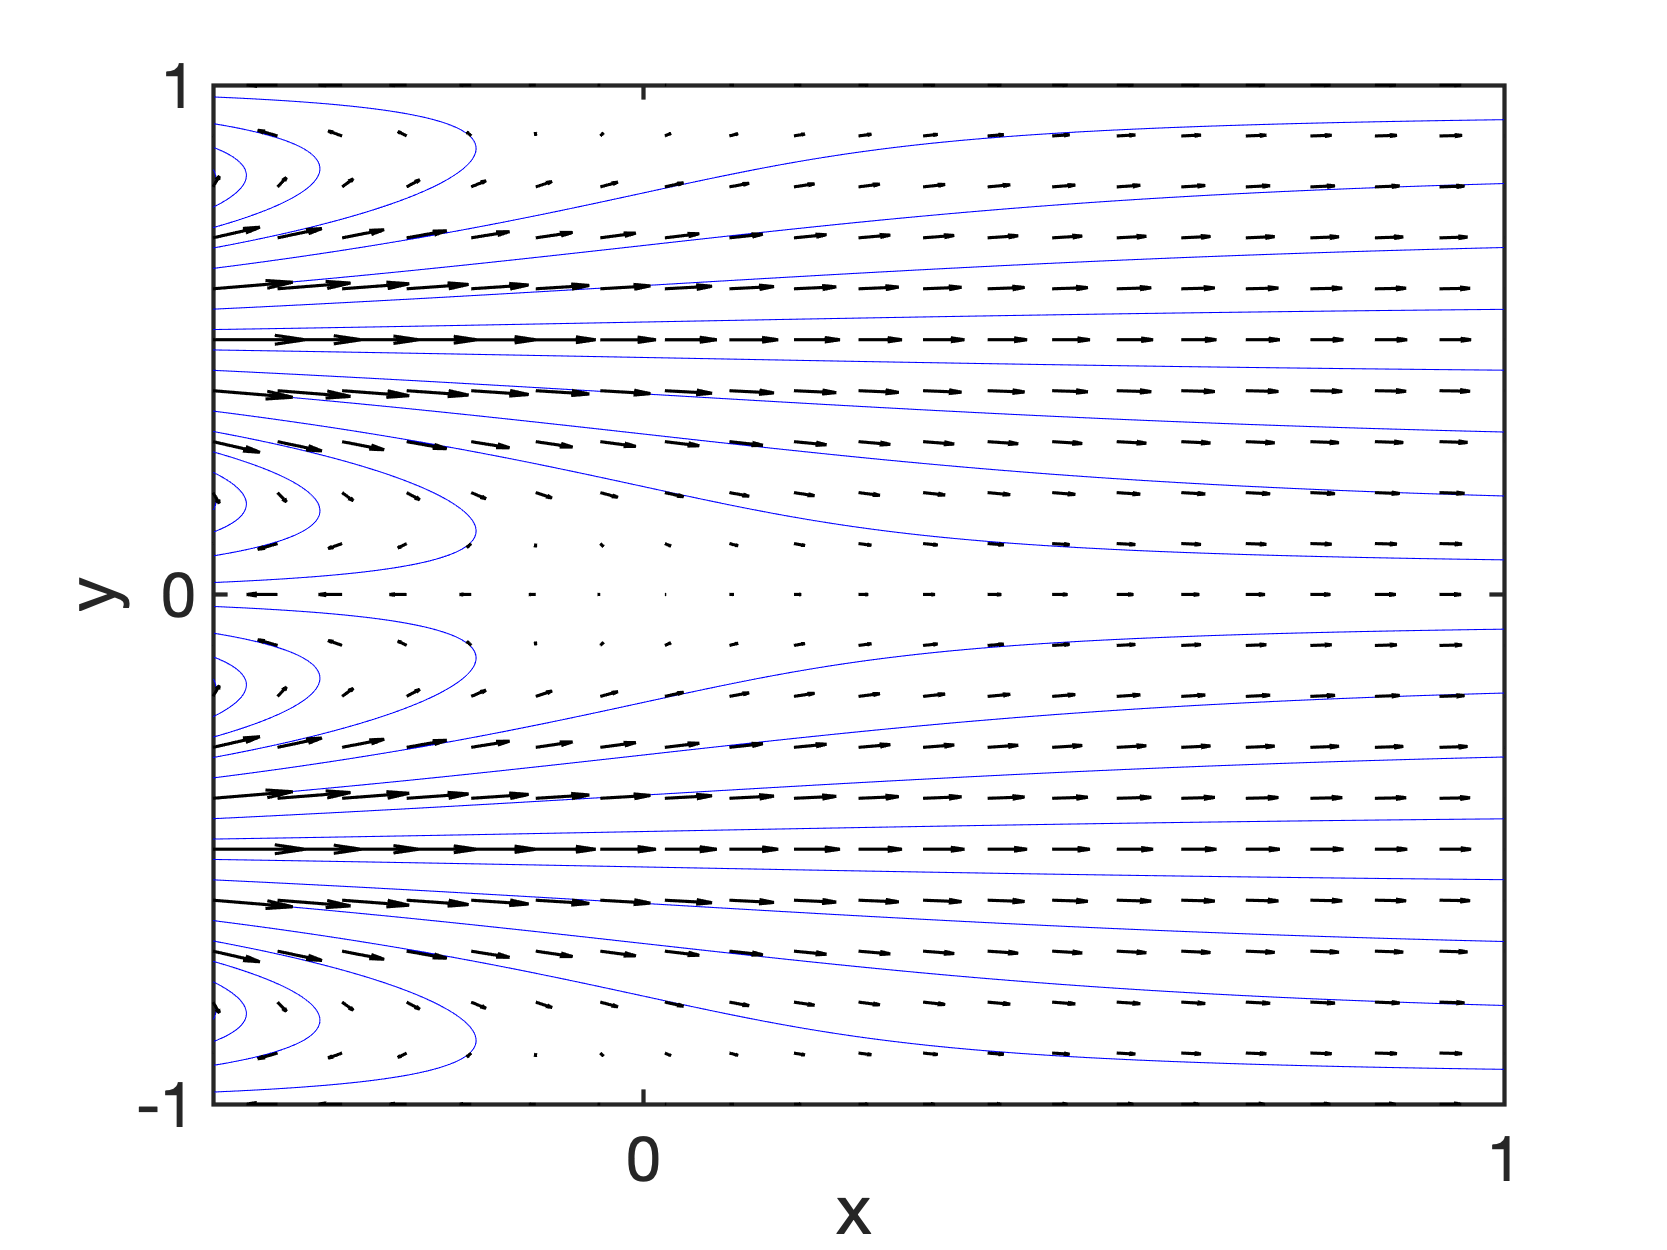
\includegraphics[scale = 0.3]{images/kovaszany}
  \caption{Streamlines and the velocity field of \eqref{eq:mms_solution_steady}.}
  \label{fig:streamlines}
\end{figure}
\begin{table}
\centering
\caption{Errors and the estimated (iterative) convergence rates of \eqref{eq:mms_solution_steady}.}
\begin{tabular}{c| cc }
 \hline
k & $\|e_k\|_\infty$ & $p$
\\
\hline
1 & 3.56e+00  & -- \\
2 & 1.85e+01  & --  \\
3 & 1.89e+00  & -1.38 \\
4 & 1.21e+00  &  0.20 \\
5 & 5.53e-01  &  1.74 \\
6 & 1.10e-01  &  2.07 \\
7 & 3.21e-03  &  2.19 \\
8 & 3.31e-06  &  1.94 \\
9 & 4.14e-12  &  1.98 \\
\hline
Theoretical && 2
\end{tabular}
\label{tab:newton_convergence}
\end{table}

Next, we move on to a more realistic case where the boundary data is set to $g_1 = 1$, $g_2 = g_3 = g_4 = g_5 = g_6 = 0$ and $\epsilon = 0.01$, which will lead to a boundary layer. The computations are performed on $\Omega = [0,1]^2$ with $200\times 200$ grid points with the SBP42 operator. \Cref{fig:boundary_layer} illustrates $\un$ for the converged solution and the iterative convergence order, $p$, is presented in \Cref{tab:boundary_layer}. The estimated iterative convergence order agrees well with what is theoretically expected. 

\begin{figure}
  \centering
  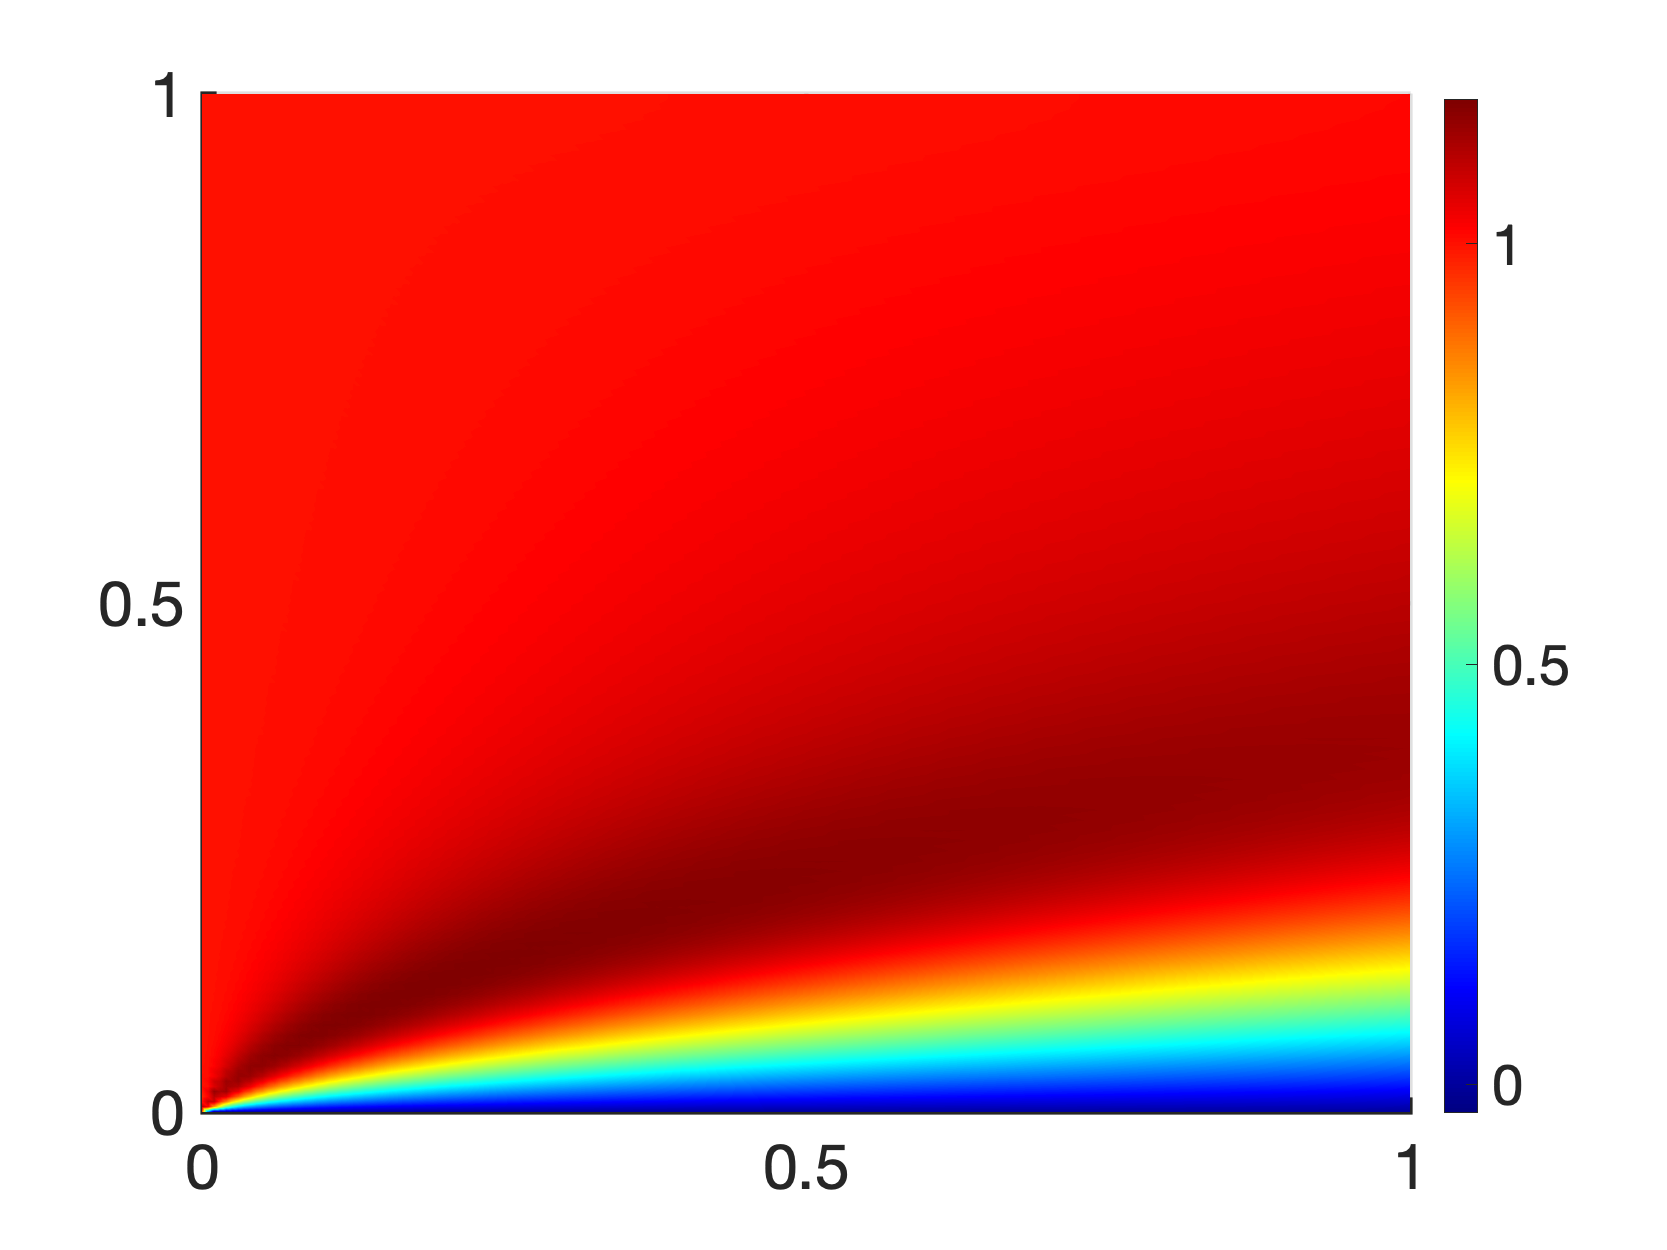
\includegraphics[scale = 0.3]{images/boundary_layer}
  \caption{Flow over a solid surface.}
  \label{fig:boundary_layer}
\end{figure}

\begin{table}
  \centering
  \caption{Errors and the estimated (iterative) convergence rates for the flow over a solid surface.}
  \begin{tabular}{c| cc }
   \hline
  k & $\|e_k\|_\infty$ & $p$
  \\
  \hline
  1 & 1.68e+00  & --  \\
  2 & 6.17e-01  & --  \\
  3 & 1.15e-01  & 1.67 \\
  4 & 4.37e-03  & 1.95 \\
  5 & 1.02e-05  & 1.85 \\
  6 & 5.51e-11  & 2.00 \\
  \hline
  Theoretical && 2
  \end{tabular}
  \label{tab:boundary_layer}
\end{table}

In the last experiment, we consider a curved grid \cite{aalund2019encapsulated} for the incompressible Euler equation (i.e. $\epsilon = 0)$. Both the south and north sides are solid surfaces, where the normal velocity is zero. The west side is an inflow boundary where $u = 1$ and $v = 0$ are specified and at the east side, $p = 0$ is imposed. We change the domain to $\Omega = [-1.5,1.5]\times [0, 0.8]$ and include a smooth bump at the south boundary given by $y(x) = 0.0625e^{-25x^2}$ \cite{bumpgrid} . In \Cref{fig:bump}, the converged solution is illustrated and the estimated iterative convergence rate $p$ is presented in \Cref{tab:bump} for the initial guess $(\un^0;\vn^0;\pn^0) = (1, \dots,1; 0, \dots ,0; 1,\dots 1)$. Again, the results agree well with the theoretical value.
\begin{figure}
 \centering
  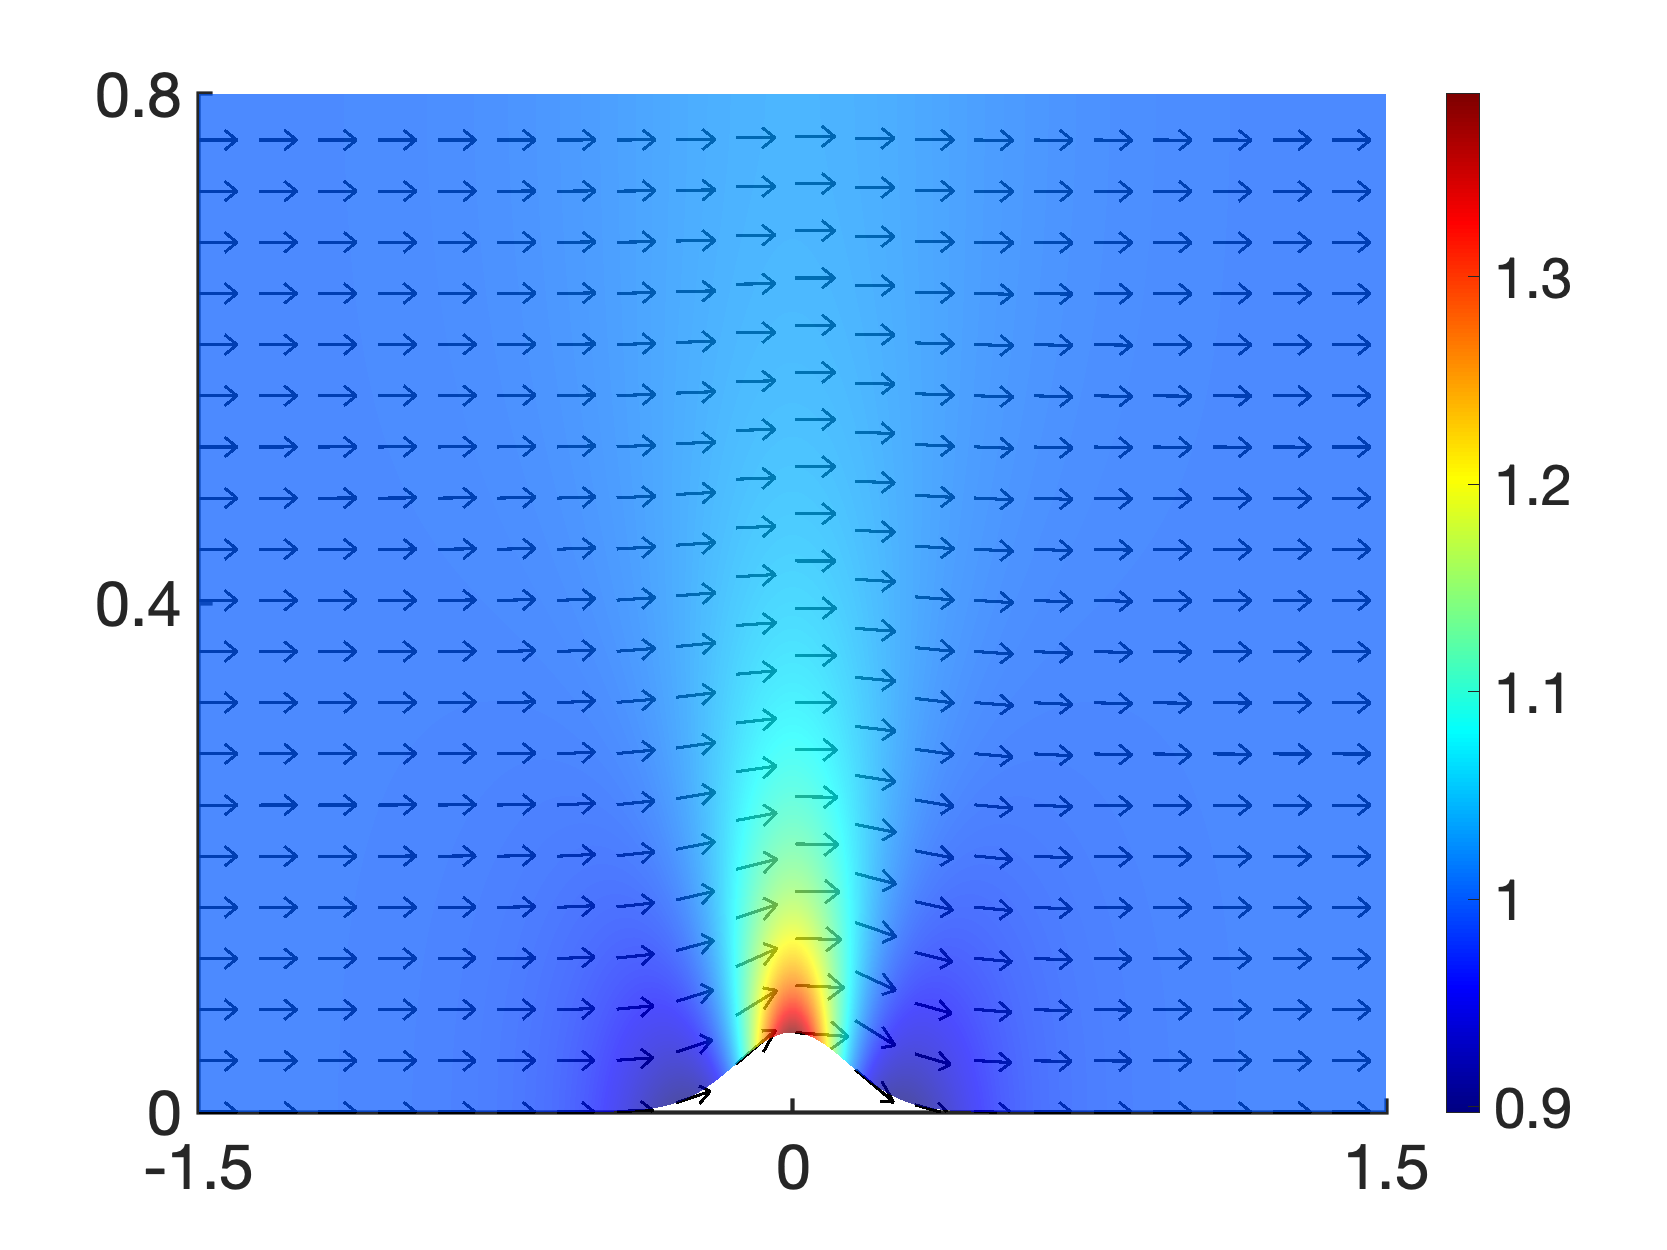
\includegraphics[scale = 0.3]{images/bump.png}
  \caption{Flow over a smooth bump. The plot illustrates the velocity field (arrows) and $\un$ (color figure) at the converged solution.}
  \label{fig:bump}
\end{figure}

\begin{table}
\centering
\caption{Errors and the estimated (iterative) convergence rates for the bump.}
\begin{tabular}{c| cc }
 \hline
k & $\|e_k\|_\infty$ & $p$
\\
\hline
1 &  3.56e+00 & --  \\
2 &  4.91e-01 & --  \\
3 &  1.74e-02 & 1.69 \\
4 &  3.33e-05 & 1.87 \\
5 &  1.55e-10 & 1.96 \\
\hline
Theoretical && 2
\end{tabular}
\label{tab:bump}
\end{table}

\section{Summary and conclusions}
We derived an explicit expression for the Jacobian of the discretization of the incompressible Euler equations. Due to the use of encapsulated difference operators, the extension to a curved grid is straight forward. Different boundary conditions such as the solid wall, the Dirichlet inflow and pressure outflow conditions have been used and the Jacobian for all these sets of boundary conditions were also presented. Lastly, the numerical method has been illustrated for different cases and also verified by the method of manufactured solutions. 


\bibliographystyle{siamplain}
\bibliography{references}

\end{document}
